\documentclass[10pt,xcolor={usenames},fleqn,mathserif,serif]{beamer}

%%%Usefull link
%tikz-equations:
%http://www.wekaleamstudios.co.uk/posts/creating-a-presentation-with-latex-beamer-equations-and-tikz/

% There are many different themes available for Beamer. A comprehensive
% list with examples is given here:
% http://deic.uab.es/~iblanes/beamer_gallery/index_by_theme.html
% You can uncomment the themes below if you would like to use a different
% one:
%\usetheme{AnnArbor}
%\usetheme{Antibes}
%\usetheme{Bergen}
%\usetheme{Berkeley}
%\usetheme{Berlin}
%\usetheme{Boadilla}
%\usetheme{boxes}
%\usetheme{CambridgeUS}
%\usetheme{Copenhagen}
%\usetheme{Darmstadt}
\usetheme{default}
%\usetheme{Frankfurt}
%\usetheme{Goettingen}
%\usetheme{Hannover}
%\usetheme{Ilmenau}
%\usetheme{JuanLesPins}
%\usetheme{Luebeck}
%\usetheme{Madrid}
%\usetheme{Malmoe}
%\usetheme{Marburg}
%\usetheme{Montpellier}
%\usetheme{PaloAlto}
%\usetheme{Pittsburgh}
%\usetheme{Rochester}
%\usetheme{Singapore}
%\usetheme{Szeged}
%\usetheme{Warsaw}

\hypersetup{pdfpagemode=FullScreen}

\addtobeamertemplate{block begin}{%
  \setlength{\textwidth}{0.95\textwidth}%
  \setlength\abovedisplayskip{0pt}%
}{}


\setbeamertemplate{caption}{\insertcaption}

%% colors
\definecolor{bittersweet}{rgb}{1.0, 0.44, 0.37}
\definecolor{brilliantlavender}{rgb}{0.96, 0.73, 1.0}
\definecolor{antiquefuchsia}{rgb}{0.57, 0.36, 0.51}
\definecolor{violetw}{rgb}{0.93, 0.51, 0.93}
\definecolor{Veronica}{rgb}{0.63, 0.36, 0.94}
\definecolor{atomictangerine}{rgb}{1.0, 0.6, 0.4}
\definecolor{darkgray}{rgb}{0.66, 0.66, 0.66}
\definecolor{brightcerulean}{rgb}{0.11, 0.67, 0.84}
\definecolor{cadmiumorange}{rgb}{0.93, 0.53, 0.18}
\definecolor{ochre}{rgb}{0.8, 0.47, 0.13}
\definecolor{midnightblue}{rgb}{0.1, 0.1, 0.44}
\definecolor{lemon}{rgb}{1.0, 0.97, 0.0}
\definecolor{grey}{rgb}{0.7, 0.75, 0.71}
\definecolor{amber}{rgb}{1.0, 0.75, 0.0}
\definecolor{almond}{rgb}{0.94, 0.87, 0.8}
\definecolor{bf}{RGB}{88, 86, 88}
\definecolor{bb}{RGB}{177, 177, 177}


%%%%%%%%%%%%%%%%%%%%%%%%%%%%%%%%%%% importa pacchetti
\usepackage{usepkg}
%%%%%%%%%%%%%%%%%%%%%%%%%%%%%%%%%%% Funzioni generali
\usepackage{functions}
%http://tex.stackexchange.com/questions/246/when-should-i-use-input-vs-include
\newcommand{\setmuskip}[2]{#1=#2\relax} %%problem usinig mu with calc (req by mathtools) loaded

\usepackage{sources}


%\usepackage{length}
%%%%%%%%%%%%%%%%%%%%%%%%%%%%%%%%%%% Funzioni per questo file main
\usepackage{mathOp}

\def\status{coazione}%ripeter
\def\keeptrying{coazione}
\usepackage{LocalF}
%%%%%%%%%%%%%%%%%%%%%%%%%%%%%%%%%

\title{Meccanica celeste (Beamer)}

% A subtitle is optional and this may be deleted
\subtitle{Moto in potenziale Newtoniano, sfera celeste, perturbazioni, determinazione orbite, ''meccanica analitica''.}

%\author{F.~Author\inst{1} \and S.~Another\inst{2}}
% - Give the names in the same order as the appear in the paper.
% - Use the \inst{?} command only if the authors have different
%   affiliation.

%\institute[Universities of Somewhere and Elsewhere] % (optional, but mostly needed)
%{
% \inst{1}
% Department of Computer Science\\
%  University of Somewhere
%  \and
%  \inst{2}%
%  Department of Theoretical Philosophy\\
%  University of Elsewhere}
% - Use the \inst command only if there are several affiliations.
% - Keep it simple, no one is interested in your street address.

\date{Dicembre, \today}
% - Either use conference name or its abbreviation.
% - Not really informative to the audience, more for people (including
%   yourself) who are reading the slides online

\subject{Orbite Kepleriane, effetti perturbativi, determinazione orbite da osservazioni, meccanica analitica. Moto dei 3 corpi.}
% This is only inserted into the PDF information catalog. Can be left
% out. 

% If you have a file called "university-logo-filename.xxx", where xxx
% is a graphic format that can be processed by latex or pdflatex,
% resp., then you can add a logo as follows:

% \pgfdeclareimage[height=0.5cm]{university-logo}{university-logo-filename}
% \logo{\pgfuseimage{university-logo}}

% Delete this, if you do not want the table of contents to pop up at
% the beginning of each subsection:
%\AtBeginPart[]
%{
%  \begin{frame}<beamer>{Outline}    %\tableofcontents[currentsection]
%  \end{frame}
%}

%\AtBeginDocument{%
%\addtolength\abovedisplayskip{-0.5\baselineskip}%
%\addtolength\belowdisplayskip{-1\baselineskip}%
%\addtolength\abovedisplayshortskip{-0.5\baselineskip}%
%\addtolength\belowdisplayshortskip{-1\baselineskip}%
%}

\makeatletter
\AtBeginPart{%
  \addtocontents{toc}{\protect\beamer@partintoc{\the\c@part}{\beamer@partnameshort}{\the\c@page}}%
}
%% number, shortname, page.
\providecommand\beamer@partintoc[3]{%
  \ifnum\c@tocdepth=-1\relax
    % requesting onlyparts.
    \makebox[6em]{PART #1:} #2
    \par
  \fi
}
\define@key{beamertoc}{onlyparts}[]{%
  \c@tocdepth=-1\relax
}
\makeatother%

\setbeamertemplate{navigation symbols}{}

\makeatletter
\setbeamertemplate{headline}
{
    \leavevmode%
    \hbox{%Refintro
        \begin{beamercolorbox}[wd=.1\paperwidth,ht=2.25ex,dp=1ex,center]{author in head/foot}%
            \hyperlink{intro}{Intro}
        \end{beamercolorbox}%

 \begin{beamercolorbox}[wd=.1\paperwidth,ht=2.25ex,dp=1ex,center]{author in head/foot}%refs Part 1
            \hyperlink{part:MSS}{MSS}
        \end{beamercolorbox}%

 \begin{beamercolorbox}[wd=.2\paperwidth,ht=2.25ex,dp=1ex,center]{author in head/foot}%refs Part 2
            \hyperlink{part:oscillations}{Oscillazioni lineari adiabatiche}
        \end{beamercolorbox}%
        
         \begin{beamercolorbox}[wd=.2\paperwidth,ht=2.25ex,dp=1ex,center]{author in head/foot}%refs Part 3
            \hyperlink{part:inverseproblem}{Problema inverso}
        \end{beamercolorbox}%inverseproblem
        
        \begin{beamercolorbox}[wd=.35\paperwidth,ht=2.25ex,dp=1ex,right]{date in head/foot}%
            %   \usebeamerfont{date in head/foot}\insertshortdate{}\hspace*{2em}
            \insertframenumber{} \hspace*{2ex}  / \hspace*{2ex} \inserttotalframenumber
            \hspace*{2ex} 
        \end{beamercolorbox}}%
        \vskip0pt%
    }
    \makeatother

\AtBeginSection{\frame{\sectionpage}}

% Let's get started
\begin{document}

\begin{filecontents}{conservedvector.tex}

\centering
\begin{figure}
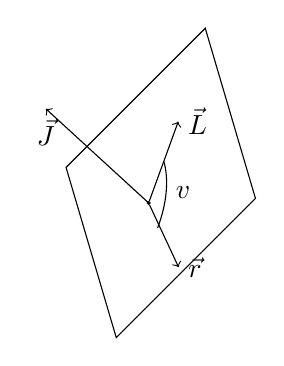
\begin{tikzpicture}[rotate around z=45, rotate around x=-45]
\draw (0,-0.3,0) -- (2.5,-0.3,0) -- (2.5,2.5,0) -- (0,2.5,0) -- cycle;
\draw[->] (1.,1.,0)node[draw,circle,inner sep=0] (o) {} -- (1.5,1.5,2)node[below] {$\vec{J}$};
\draw[->] (o) -- ++(295:0.9cm)node[right] {$\vec{r}$};
\draw[->] (o) -- ++(70:1.1cm)node[right] {$\vec{L}$}node [midway] (aux){};
\draw (aux) arc (0:-50:1) node[midway,right] {$v$};
\end{tikzpicture}

\label{fig:Lenztikz}

\end{figure}

\end{filecontents}


\begin{filecontents}{reducedproblem.tex}
%reduced problem
\begin{tikzpicture}

\node[circle,fill,inner sep=1pt,label=above:$m_1$] (M) at (0,0) {}; 
\draw (M)--++(30:1cm) node[circle,fill,inner sep=1pt,label=below:O] (O) {};
\draw[->] (O)--++(30:1.5cm) node[circle,fill,inner sep=1pt,label=above:$m_2$,yshift=1pt,xshift=1pt] (m) {} node[midway,above] {$\vec{r}$} ;

\node[circle,fill,inner sep=1pt,below=1cm of O,label=below:O] (O1) {}; 
\draw[->] (O1)--++(30:1.5cm) node[circle,fill,inner sep=1pt,label=above:$m_2$,yshift=1pt,xshift=1pt] (m1) {} node[midway,below] {$\vec{r_1}$} ;
\draw[->] (O1)--++(-150:1cm) node[circle,fill,inner sep=1pt,label=above:$m_1$,yshift=1pt,xshift=1pt] (m1) {} node[midway,below] {$\vec{r_2}$} ;
%\node (dida) at (7,0) {\parbox{8cm}{Siano m e M due masse puntiformi o a simmetria sferica: O \'e il centro di massa e $\vec{r}=\vec{r_1}-\vec{r_2}$ la distanza relativa.}};

\end{tikzpicture}

\end{filecontents}

\begin{filecontents}{ellipse.tex}

%ellisse

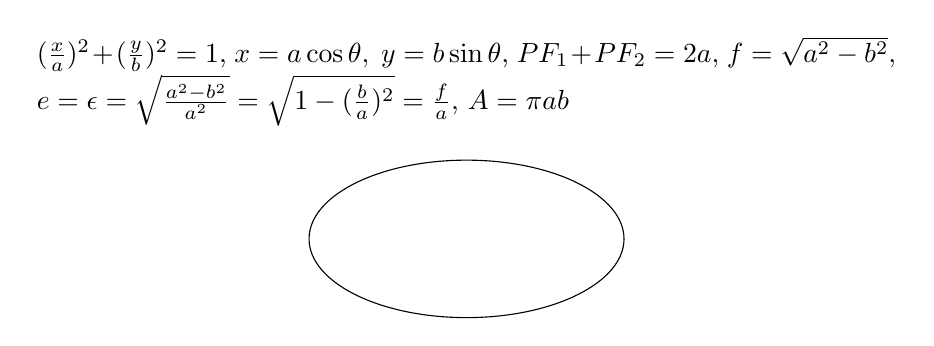
\begin{tikzpicture}

\draw ellipse (2cm and 1cm) node (o) {};
\node (prop) at (0,2) {\parbox{0.9\textwidth}{
$(\frac{x}{a})^2+(\frac{y}{b})^2=1$,
$x=a\cos{\theta},\ y=b\sin{\theta}$,
$PF_1+PF_2=2a$,
$f=\sqrt{a^2-b^2}$,
$e=\epsilon=\sqrt{\frac{a^2-b^2}{a^2}}=\sqrt{1-(\frac{b}{a})^2}=\frac{f}{a}$,
$A=\pi ab$}
};

\end{tikzpicture}

\end{filecontents}%%contain tikz files as filecontents

\addtobeamertemplate{block begin}{\setlength\abovedisplayskip{2pt}\setlength\belowdisplayskip{2pt}\setlength\abovedisplayshortskip{2pt}\setlength\belowdisplayshortskip{2pt}}

\addtobeamertemplate{block begin}{\vspace*{-3pt}}{}
\addtobeamertemplate{block end}{}{\vspace*{-3pt}}

\begin{frame}
  \titlepage
\end{frame}

% Section and subsections will appear in the presentation overview
% and table of contents.
%\frame{\tableofcontents[onlyparts]}

\begin{frame}[label={argomenti}]{Sistemi planetari: argomenti del corso}

\tableofcontents[onlyparts]


\end{frame}

\begin{wordonframe}{orbite, fenomenologia formazione}

Orbite dei corpi celesti: problema Kepleriano, problema a 3 corpi, problema multicorpi: perturbazioni.

\end{wordonframe}


\part{Moto 2 corpi in potenziale newtoniano}\label{part:kepler}
\frame{\partpage}

\begin{frame}{this part toc}

\begin{itemize}

\item Problema ridotto: Potenziale newtoniano/ Esistenza orbite chiuse
\item costanti del moto
\item leggi di Keplero
\item Traiettoria o legge oraria
\item elementi orbitali
\item approssimazione piccola eccentricit\'a
\item determinazione orbita pianeta orbitante attorno al Sole da 3 osservabili

\end{itemize}

\end{frame}

\section{Orbite Kepleriane}

\begin{frame}{Problema ridotto}

\begin{columns}

\begin{column}{0.55\textwidth}

\input{reducedproblem}

\end{column}

\begin{column}{0.45\textwidth}

\end{column}

\end{frame}

\section{Determinazione orbita da 3 osservabili (Solar system)}\label{sec:orbitobs}

\section{Definizione del problema}

\begin{frame}{Necessarie 3 osservazioni}

\begin{columns}

\begin{column}{0.3\textwidth}

\begin{figure}[!ht]

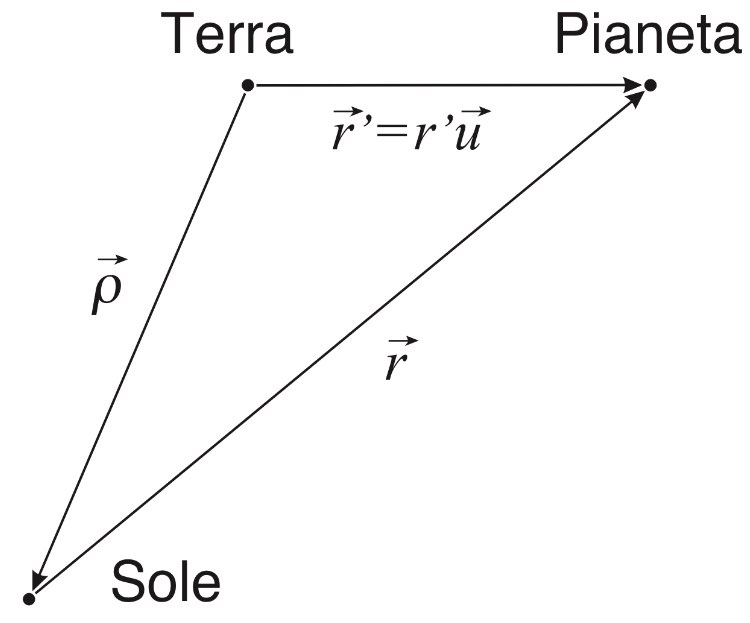
\includegraphics[width=\textwidth]{iterationorbit}

\end{figure}

\end{column}

\begin{column}{0.7\textwidth}

\begin{align*}
&\alpha_1=\alpha_1(i,\omega,\Omega,\chi,a,e,\phi_0;t_1)\\
&\delta_1=\delta_1(i,\omega,\Omega,\chi,a,e,\phi_0;t_1)\\
&\alpha_2=\alpha_2(i,\omega,\Omega,\chi,a,e,\phi_0;t_2)\\
&\delta_2=\delta_2(i,\omega,\Omega,\chi,a,e,\phi_0;t_2)\\
&\alpha_3=\alpha_3(i,\omega,\Omega,\chi,a,e,\phi_0;t_3)\\
&\delta_3=\delta_3(i,\omega,\Omega,\chi,a,e,\phi_0;t_3)
\end{align*}

\end{column}

\end{columns}

\begin{block}{Metodo iterativo}
da una soluzione approssimata ne ricaviamo una pi\'u corretta
\end{block}

\end{frame}

\begin{frame}{Metodo di Laplace}


\end{frame}


\begin{frame}{Metodo di Gauss}


\end{frame}


\part{Problema Newtoniano: meccanica analitica.}\label{part:analitic}

\begin{frame}{this part toc}

\begin{itemize}

\item Meccanica analitica: equazione di H-J, separazione di H-J, e soluzione
\item variabili canoniche
\item azione ridotta
\item Teorema di Liouville-Arnold: soluzione equazioni del moto tramite quadratura
\item degenerazione periodi orbitali

\end{itemize}


\end{frame}

\section{Equazioni di Hamilton}\linkdest{Hameqs}
\begin{frame}{Hamiltoniana problema 2 corpi ridotto}
\begin{columns}
\begin{column}{0.2\textwidth}
\begin{figure}[!ht]
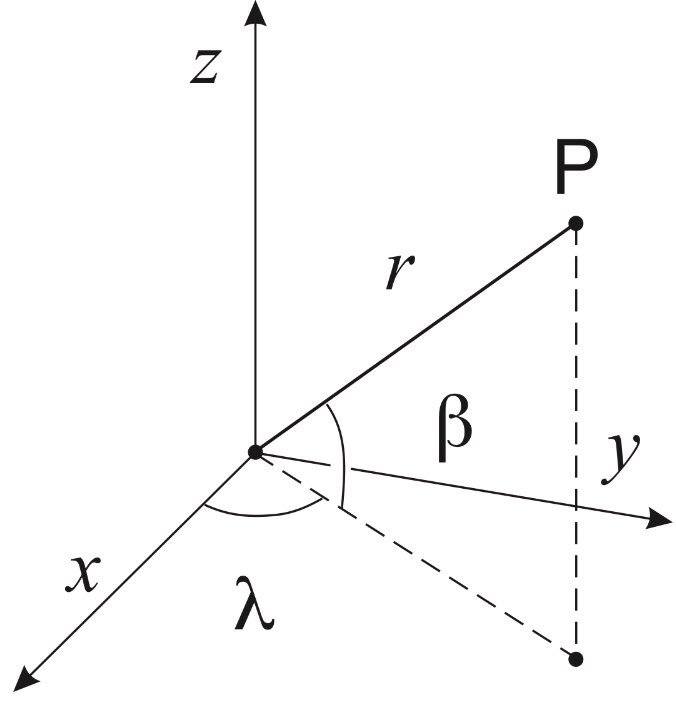
\includegraphics[width=\textwidth]{analytic}
\end{figure}
\end{column}
\begin{column}{0.8\textwidth}
\begin{align*}
&T=\frac{1}{2}\mu(\dot{r}^2+r^2\dot{\beta}^2+r^2\cos^2{\beta}\dot{\lambda}^2)\\
&V=-k^2\frac{\mu}{r}\\
&L=T-V
\end{align*}
\end{column}
\end{columns}
\begin{block}{Momenti coniugati}
\begin{align*}
&p_r=\PDy{\dot{r}}{L}=\mu\dot{r}\\
&p_{\beta}=\PDy{\dot{\beta}}{L}=\mu r^2\dot{\beta}\\
&p_{\lambda}=\PDy{\dot{\lambda}}{L}=\mu r^2\cos^2{\beta}\dot{\lambda}\quad \dot{p}_{\lambda}=0
\end{align*}
\end{block}
\begin{block}{Hamiltoniana}
\begin{align*}
&H(p,q)=\frac{1}{2\mu}(p_r^2+\frac{1}{r^2}p_{\beta}^2+\frac{1}{r^2\cos^2{\beta}}p_{\lambda}^2)-\frac{k^2\mu}{r}
\end{align*}
\end{block}
\end{frame}

\begin{wordonframe}{Meccanica Hamiltoniana}
\begin{block}{Equazioni di Hamilton}
\begin{align*}
&\dot{q}=\PDy{p}{H}\\
&\dot{p}=-\PDy{q}{H}
\end{align*}
\end{block}
$\TDy{t}{H}=\PDy{t}{H}$
\end{wordonframe}

\section{Equazione di Hamilton-Jacobi}\linkdest{HJeqs}

\begin{frame}{Problema di H-J}
\begin{block}{Trasformazioni canoniche}
\begin{align*}
(p,q)\to(\xi(p,q),\eta(p,q))
\end{align*}
che lasciano invariate le equazioni di Hamilton.
\end{block}
\begin{block}{Problema di H-J}
Trovare trasformazione canonica tale che $K=0$: $(\xi,\eta)$ sono costanti del moto.
\end{block}
\begin{block}{Funzione generatrice $S(q,\eta,t)$}
\begin{align*}
&\xi=\PDof{\eta}S(q,\eta,t)\ (2: \xi(p,q))\\
&p=\PDof{q}S(q,\eta,t)\ (1:\eta(q,p))\\
&K=H+\PDy{t}{S}\ K=0\Leftrightarrow H(q,\PDy{q}{S},t)=-\PDy{t}{S}
\end{align*}
\end{block}
\end{frame}

\begin{frame}{Soluzione dell'equazione di H-J}
\begin{align*}
\frac{1}{2\mu}[(\PDy{r}{S})^2+\frac{1}{r^2}(\PDy{\beta}{S})^2+\frac{1}{r^2\cos^2{\beta}}(\PDy{\lambda}{S})^]-\frac{k^2\mu}{r}=-\PDy{t}{S}
\end{align*}
Un integrale completo contiene tante variabili quanti sono i gradi di libert\'a: le $\eta$.
\begin{block}{L'equazione di H-J \'e separabile}
\begin{columns}
\begin{column}{0.5\textwidth}
Variabili canoniche $J_{\phi}, J_{\chi}, J_{\psi}$:
\begin{equation*}
S=J_{\phi}(u+e\sin{u})+J_{\chi}\chi+J_{\psi}\psi-Et
\end{equation*}
\end{column}
\begin{column}{0.5\textwidth}
Variabili canoniche $E, J, J_{\lambda}$:
\begin{equation*}
S(r,\beta,\lambda,t)=S_r(r)+S_{\beta}(\beta)+S_{\lambda}(\lambda)-\sigma t
\end{equation*}
\end{column}
\end{columns}
\end{block}
\end{frame}

\begin{wordonframe}{Canonical var}
\begin{columns}\begin{column}{0.5\textwidth}
\begin{align*}
&\PDy{J_{\phi}}{S}=\phi-nt\\
&\PDy{J_{\chi}}{S}=w-v=\chi\\
&\PDy{J_{\psi}}{S}=\lambda-\bar{\lambda}=\psi
\end{align*}
\end{column}\begin{column}{0.5\textwidth}
\begin{align*}
&S_{\lambda}=J_{\lambda}\lambda\\
&S_{\beta}=Jw-J_{\lambda}\bar{\lambda}\\
&S_r=ku\sqrt{a}(u+e\sin{u})-ku\sqrt{p}v\\
&\PDy{E}{S_r}=\frac{\phi}{n} \ \PDy{J}{S_r}=-v
\end{align*}
\end{column}\end{columns}
\end{wordonframe}


\section{Sistemi integrabili e degenerazione}\linkdest{intdeg}

\begin{frame}{Teorema di Liuville-Arnol'd}
Se in un sistema Hamiltoniano con n gradi di libert\'a sono noti n integrali primi del moto indipendenti ed in involuzione (parentesi di Poisson nulle) allora esiste una trasformazione canonica nelle variabili angolo-azione nella quale H dipende solo dalle variabili azione mentre le variabili angolo evolvono linearmente nel tempo. Le equazioni del moto potranno essere risolte tramite quadratura.
\end{frame}

\begin{wordonframe}{Integrabilit\'a EOM}
\begin{align*}
\frac{dq_1}{\sqrt{2(hf_1-v_1+c_1)}}=\ldots=\frac{dq_n}{\sqrt{2(hf_n-v_n+c_n)}}=\frac{dt}{f}=d\tau
\end{align*}
\end{wordonframe}

\begin{frame}{Periodi del moto}
Quando i periodi indipendenti sono meno dei gradi di libert\'a si parla di degenerazione: \'e connessa con la possibilit\'a di scegliere in pi\'u modi le 3 costanti del moto del teorema di L-A.
\end{frame}


\part{Attrazione non Newtoniana, orbite non Kepleriane: perturbazioni.}\label{part:perturbation}

\begin{frame}{this part toc}

\begin{itemize}

\item Potenziale non-Newtoniano: perturbazioni orbite non Kepleriane
\item Sviluppi in multipoli dell'energia potenziale
\item Moto perturbato
\item Metodo di Neton
\item Precessione luni-solare
\item Perturbazioni degli elementi orbitali: periodiche e secolari
\item Analogo quantistico
\item Elementi osculanti

\end{itemize}

\end{frame} 

\section{Primario non sferico}

\begin{frame}{Sviluppo in multipoli energia potenziale}

\begin{align*}
V(\vec{r})=-\frac{Gm}{r}[\int\rho'\,d^3r'+\cos{\theta}\int\frac{r'}{r}\cos{\theta'}\rho(\vec{r}')\,d^3r'\\
+\frac{1}{2}(3\cos^2{\theta}-1)\int\frac{r'}{r}\frac{1}{2}(3\cos^2{\theta}-1)\rho(\vec{r}')\,d^3r'+\ldots]
\end{align*}

\begin{block}{Potenziale di quadrupolo}

\begin{equation*}
V(\vec{r})=-\frac{Gm}{r}[M+\frac{1}{2r^2}(A-C)(3\cos^2{\theta}-1)+\ldots]
\end{equation*}

\end{block}

\end{frame}

\begin{wordonframe}{Momento inerzia e $J_2$}

\begin{align*}
&I_x=I_y=A=\int(x'^2+z'^2)\rho\,d^3r'=\int(y'^2+z'^2)\rho\,d^3r'\\
&I_z=C=\int(x'^2+y'^2)\rho\,d^3r'\\
&J_2=\frac{C-A}{MR^2}\, GmM=k^2\mu\\
\end{align*}

$J_2>0$ for any planet flatten by rotation

\begin{block}{Terra-Luna}

\begin{align*}
J_2^{\oplus}\approx\num{e-3}\\
(\frac{R}{r})^2\approx(\frac{1}{60})^2\approx\num{3e-4}\\
\frac{V_Q}{V_N}\approx\num{3e-7}
\end{align*}

\end{block}

\end{wordonframe}

\begin{frame}{Forza perturbatrice}

\begin{columns}
\begin{column}{0.6\textwidth}

\begin{align*}
&V=-\frac{k^2\mu}{r}+V'\\
&V'=-\frac{3Q}{r^5}(\frac{1}{3}-\cos^2{\theta})\\
&Q=\frac{1}{2}k^2\mu R^2J_2
\end{align*}

\end{column}
\begin{column}{0.4\textwidth}

\begin{figure}[!ht]
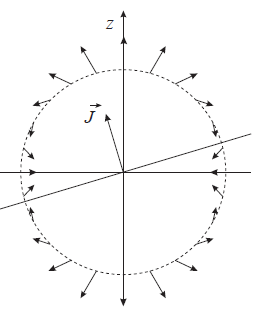
\includegraphics[width=\textwidth]{perturbation}
\end{figure}

\end{column}
\end{columns}

$e$, $i$, $|\vec{J}|$ non variano in media su un periodo.

\begin{block}{Periodo del moto radiale (i=0)}

Traiettoria a ''rosetta'':

\begin{equation*}
T_{\lambda}=\frac{\pi}{\Delta}T_{r}
\end{equation*}

\end{block}

\end{frame}

\begin{wordonframe}{forza perturbatrice}

\begin{align*}
&f_x=3Qr\expy{-4}(5\cos^2{\theta}-1)\sin{\theta}\cos{\lambda}\\
&f_y=3Qr\expy{-4}(5\cos^2{\theta}-1)\sin{\theta}\sin{\lambda}\\
&f_z=3Qr\expy{-4}(5\cos^2{\theta}-1)\cos{\theta}
\end{align*}

\begin{block}{Integrali primi del moto ($i=0$)}
\begin{align*}
&\mu r^2\dot{\lambda}^2=J\\
&\frac{1}{2}\mu\dot{r}^2-\frac{k^2\mu}{r}+\frac{J^2}{2\mu r^2}+V'=E
\end{align*}
\end{block}

\begin{align*}
&T_r=2\int_{r_{min}}^{r_{max}}\,dr(\frac{2E}{\mu}-\frac{2V'}{\mu}-\frac{J^2}{\mu^2r^2}+\frac{2k^2}{r})\expy{-\frac{1}{2}}\\
&\Delta=\frac{J}{\mu}\int_{r_{min}}^{r_{max}}\,dr(\frac{2E}{\mu}-\frac{2V'}{\mu}-\frac{J^2}{\mu^2r^2}+\frac{2k^2}{r})\expy{-\frac{1}{2}}
\end{align*}

\end{wordonframe}

\begin{frame}{Effetti su orbita}

\begin{itemize}
\item Linea dei nodi regresses for prograde orbit ($i\neq\pi/2$) - Piano orbita ruota backward

\item $\forall i<\ang{46.5}$ il pericentro ruota in avanti.

\item $\forall i<\sin{\sqrt{\frac{2}{3}}}\expy{-1}=\ang{54.7}$ mean anomaly increases at rate greater than n: orbital period is less then for keplerian orbit about spherical planet of same mass.

\item We can determine $J_2$ for planets having satellites in eccentric/inclined orbit.

\end{itemize}

\end{frame}

\section{Metodo di Newton}


\begin{equation*}
\mu\ddot{r}=f+\frac{c}{r^3}+\frac{J^2}{\mu r^3}=f+\frac{J'^2}{\mu r^3}
\end{equation*}


Stessa moto radiale con diverso j; moto angolare perturbato ha velocit\'a proporzionale a quello imperturbato: $\frac{\dot{\lambda}}{\dot{\lambda'}}=\frac{J}{J'}$.

\begin{block}{Orbita quasi-circolare}
Moto medio del pericentro: $\frac{3}{2}n\frac{R^2}{a^2}J_2$.
\end{block}

\begin{wordonframe}{Perturbazione orbita quasi-circolare}

f forza centrale

\begin{align*}
V'(\theta=\pi/2)=-\frac{3Q}{r^4}\approx\frac{3Q}{r^2a^2}-\frac{6Q}{ar^3}+o((r-a)^2)
\end{align*}

\end{wordonframe}

\section{Precessione luni-solare}

\begin{frame}{Momento rispetto al CM della Terra}

\begin{columns}  \begin{column}{0.3\textwidth}

\begin{figure}[!ht]

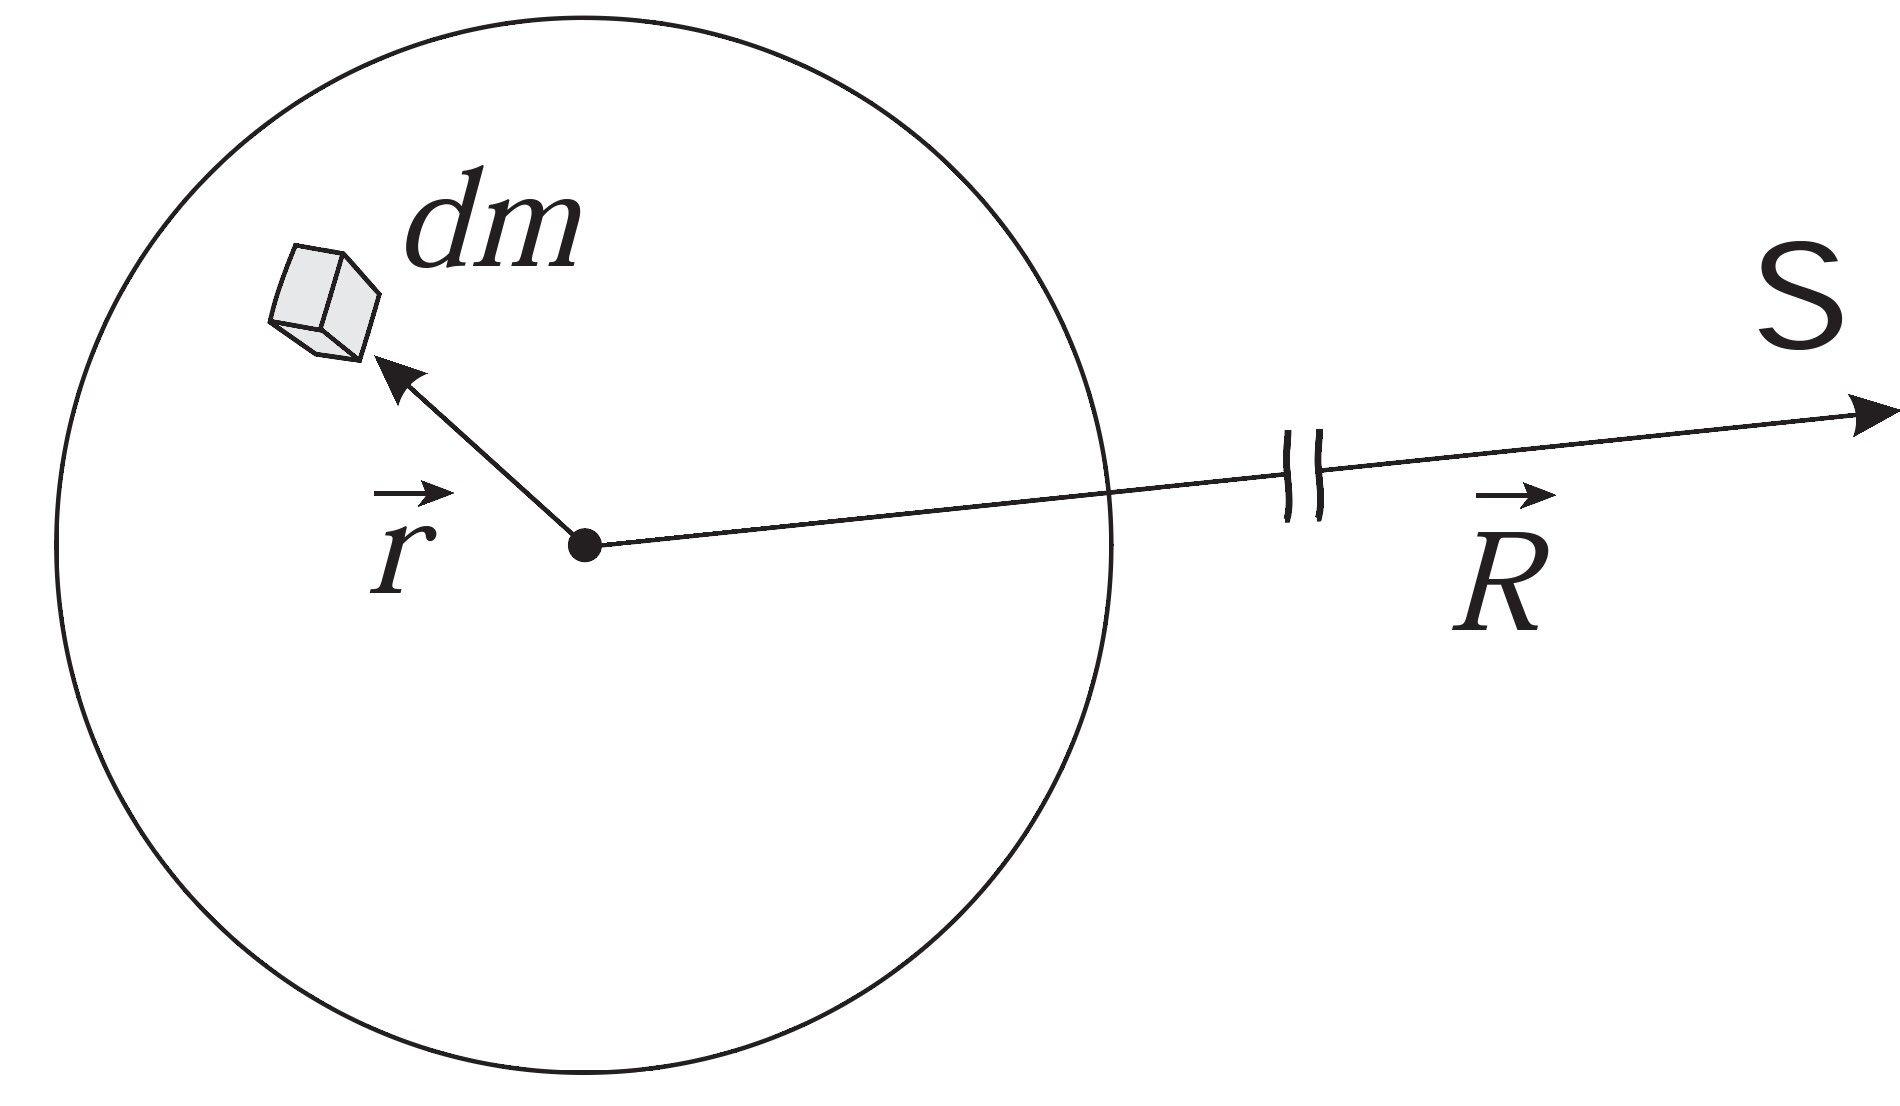
\includegraphics[width=\textwidth]{Sunearth}

\end{figure}

\end{column} \begin{column}{0.7\textwidth}

\begin{equation*}
d\vec{K}=\vec{r}\wedge d\vec{F}=\frac{GM\,dm}{R^3}(1+3\frac{\scap{R}{r}}{R^2})\vecp{r}{R}
\end{equation*}

\end{column}  \end{columns}

\begin{block}{Media annua}

\begin{columns}  \begin{column}{0.4\textwidth}

\begin{align*}
&\bar{K}_{\xi}=\frac{3GM}{2R^3}(C-A)\sin{\epsilon}\cos{\epsilon}\\
&\bar{K}_{\eta}=\bar{K}_{\zeta}=0
\end{align*}

\end{column} \begin{column}{0.6\textwidth}

\begin{figure}[!ht]

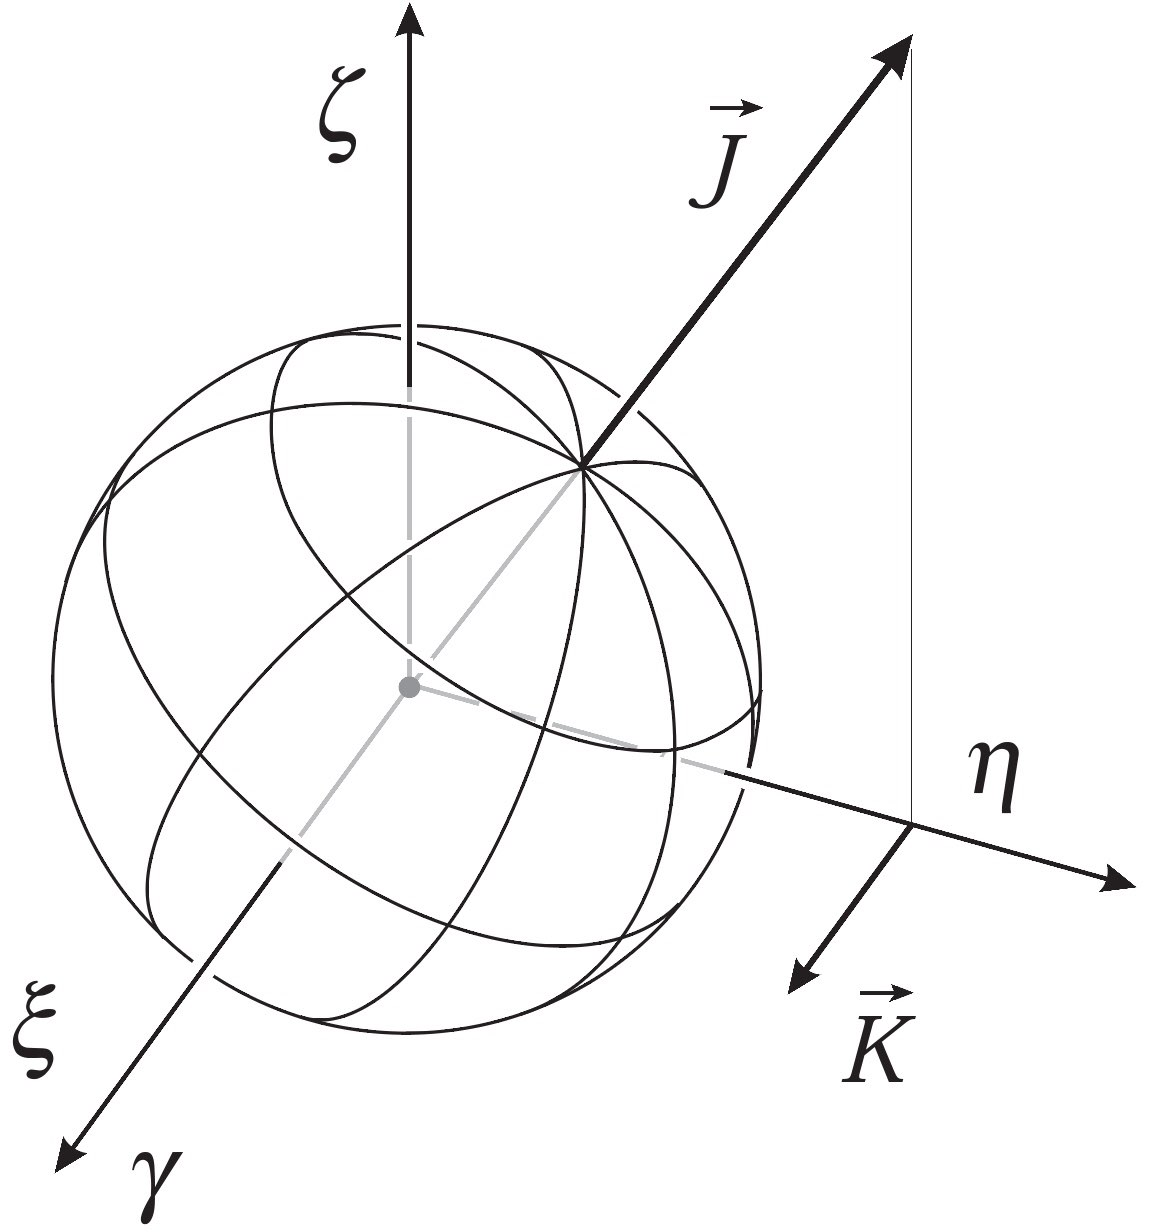
\includegraphics[width=0.5\textwidth]{eclcoord}

\end{figure}

\end{column}
\end{columns}

\end{block}

\begin{block}{Velocit\'a di precessione della Terra dovuta all'attrazione lunisolare}

\begin{equation*}
P=P_{\odot}+P_{\leftmoon}\approx\ang{;;50.3}\si{\per\year}
\end{equation*}


\end{block}


\end{frame}

\begin{wordonframe}{Precessione lunisolare}

Coordinate eclittiche: $\lambda$ longitudine eclittica del Sole, $\epsilon$ obliquit\'a dell'eclittica

\begin{block}{Momento delle forze}

\begin{align*}
&K_x=\frac{3GM}{2R^5}(C-A)YZ\\
&K_y=\frac{3GM}{2R^5}(C-A)XZ\\
&K_z=0
\end{align*}

\end{block}

\begin{block}{Poisson's relations}

\begin{equation*}
(\TDy{t}{\vec{u}})_{fix}=(\TDy{t}{\vec{u}})_{rot}+\vecp{\omega}{u}
\end{equation*}

\end{block}

\end{wordonframe}


\section{Perturbazioni}

\begin{frame}{Meccanica analitica}

\begin{columns}  \begin{column}{0.5\textwidth}

\begin{block}{Approssimazione di quadrupolo}

\begin{align*}
&H=H_0+H_1\\
&H_0=-\frac{k^4\mu^3}{2J_{\phi}^2}\\
&H_1=\frac{3}{2}R^2J_2k^2\mu\frac{1}{r^3}(\sin^2{\beta}-\frac{1}{3})
\end{align*}


\end{block}

\end{column}

\begin{column}{0.5\textwidth}

\begin{block}{Simmetria cilindrica}

\begin{equation*}
\dot{J_{\psi}}=\PDy{\psi}{H}=0
\end{equation*}

Componente lungo z del momento angolare costante.

\end{block}


\end{column}  \end{columns}


\end{frame}



\begin{wordonframe}{Soluzione imperturbata}

\begin{block}{Costanti del moto}

\begin{equation*}
J_{\phi}, J_{\chi}, J_{\psi}, \chi, \psi
\end{equation*}


\end{block}


Variabili canoniche: $\phi$, $\chi$, $\psi$, $J_{\phi}$, $J_{\chi}$, $J_{\psi}$

\begin{align*}
&\sin{\beta}=\sin{i}\sin{w}\ \cos{i}=\frac{J_{\psi}}{J_{\chi}}\ w=\chi+v\\
&v(\phi,e)\ e(J_{\phi},J_{\chi})
\end{align*}

$\phi$ anomalia media


\begin{equation*}
\dot{\phi}=\PDy{J_{\phi}}{H_0}=n
\end{equation*}



\end{wordonframe}



\begin{frame}{Termine perturbativo in funzione delle variabili canoniche}


\begin{block}{Prim'ordine}

Soluzioni imperturbate per $\beta$ e r periodiche: il termine $\frac{1}{r^3}(\sin^2{\beta}-\frac{1}{3})$ \'e periodico.

\begin{equation*}
H_1=A_0+\sum_{h=1}^{\infty}A_h\cos{h\phi}+\sum_{h=1}^{\infty}B_k\sin{h\phi}
\end{equation*}


\end{block}

\begin{block}{Perturbazioni periodiche}

\begin{align*}
&-\dot{J_{\phi}}=\PDy{\phi}{H}=\PDy{\phi}{H_1}=-\sum_hhA_h\sin{(h\phi)}+\sum_hhB_h\cos{(h\phi)}\\
&-\dot{J_{\chi}}=\PDy{\chi}{H}=\PDy{\chi}{H_1}=-\sum_h\PDy{\chi}{A_h}\sin{(h\phi)}+\sum_h\PDy{\chi}{B_h}\cos{(h\phi)}
\end{align*}


\end{block}

\end{frame}


\begin{frame}{Perturbazioni secolari}

\begin{align*}
&\dot{\phi}=\PDy{J_{\phi}}{H_0}+\PDy{J_{\phi}}{H_1}\approx n(1+\frac{3R^2}{4a^2}J_2\frac{2-3\sin^2{i}}{(1-e^2)\expy{\frac{3}{2}}})\\
&\dot{\chi}\approx n\frac{3R^2}{4a^2}J_2\frac{4-5\sin^2{i}}{(1-e^2)^2}\\
&\dot{\psi}\approx-n\frac{3R^2}{2a^2}J_2\frac{\cos{i}}{(1-e^2)^2}
\end{align*}


\end{frame}

\begin{wordonframe}{Calcolo esplicito perturbazione secolare}

\begin{align*}
\bar{H}_1=\frac{1}{2\pi}\int_0^{2\pi}H_1\,d\phi
\end{align*}

\end{wordonframe}


\begin{frame}{Perturbazioni secolari: $i=0$}

\begin{figure}[!ht]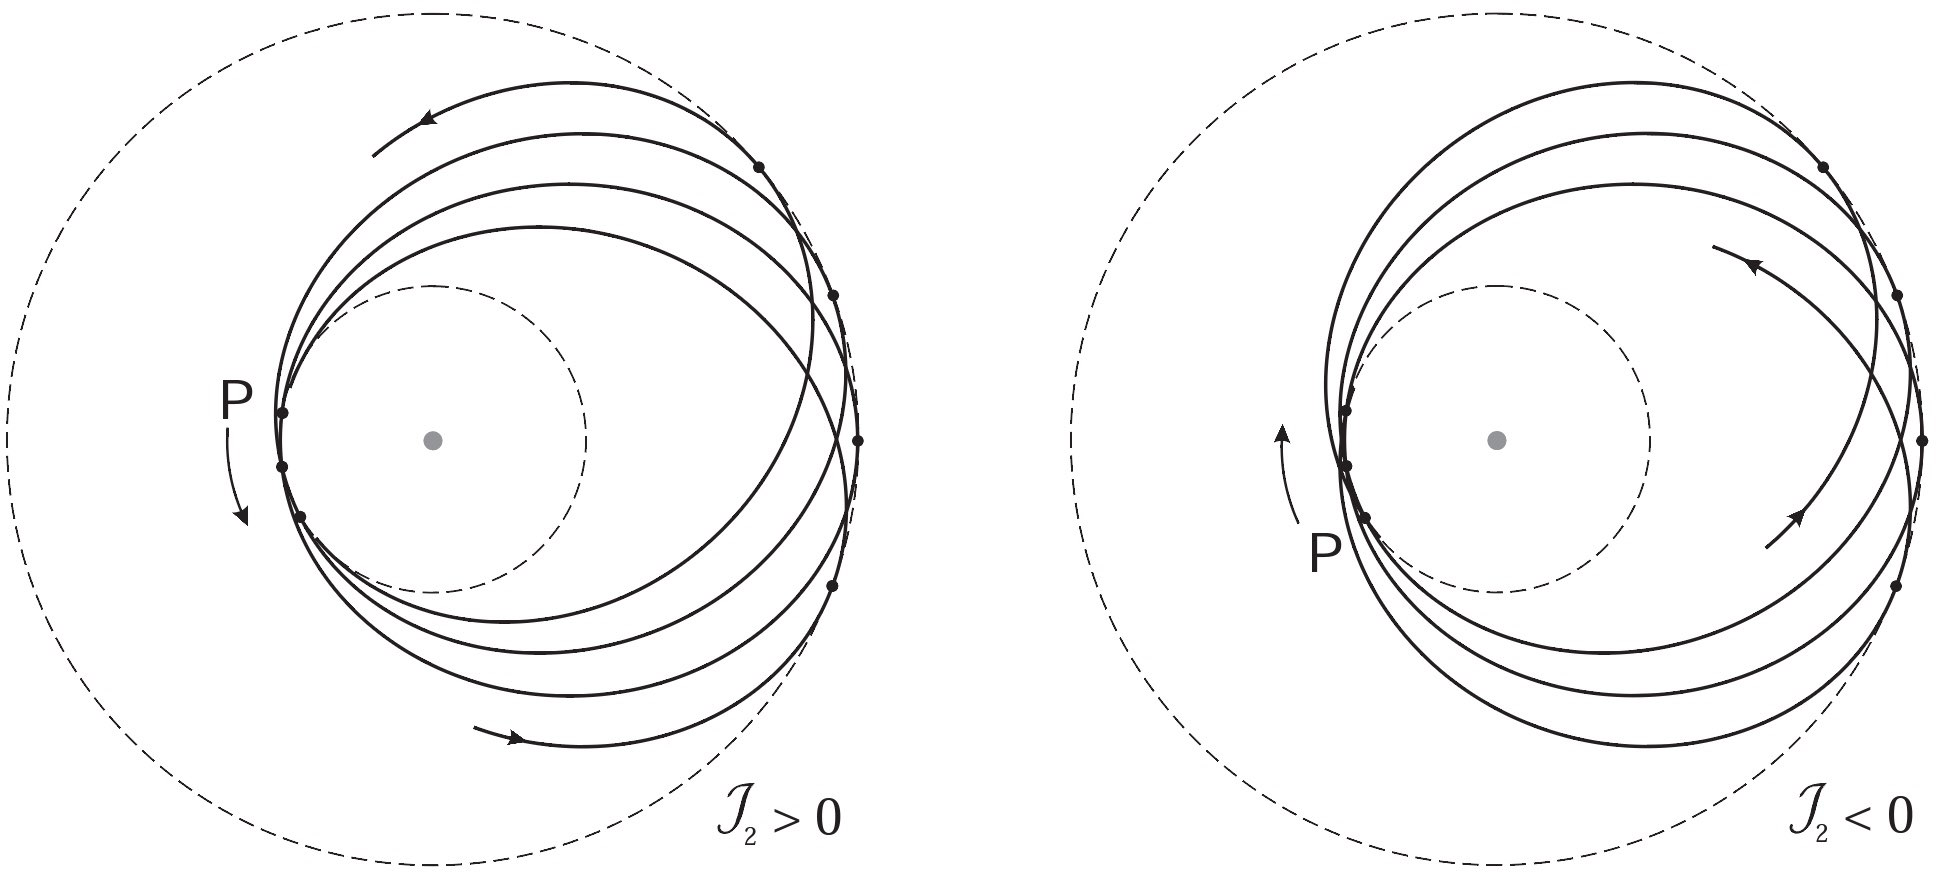
\includegraphics[height=0.4\textheight]{peripert}\end{figure}

\begin{figure}[!ht]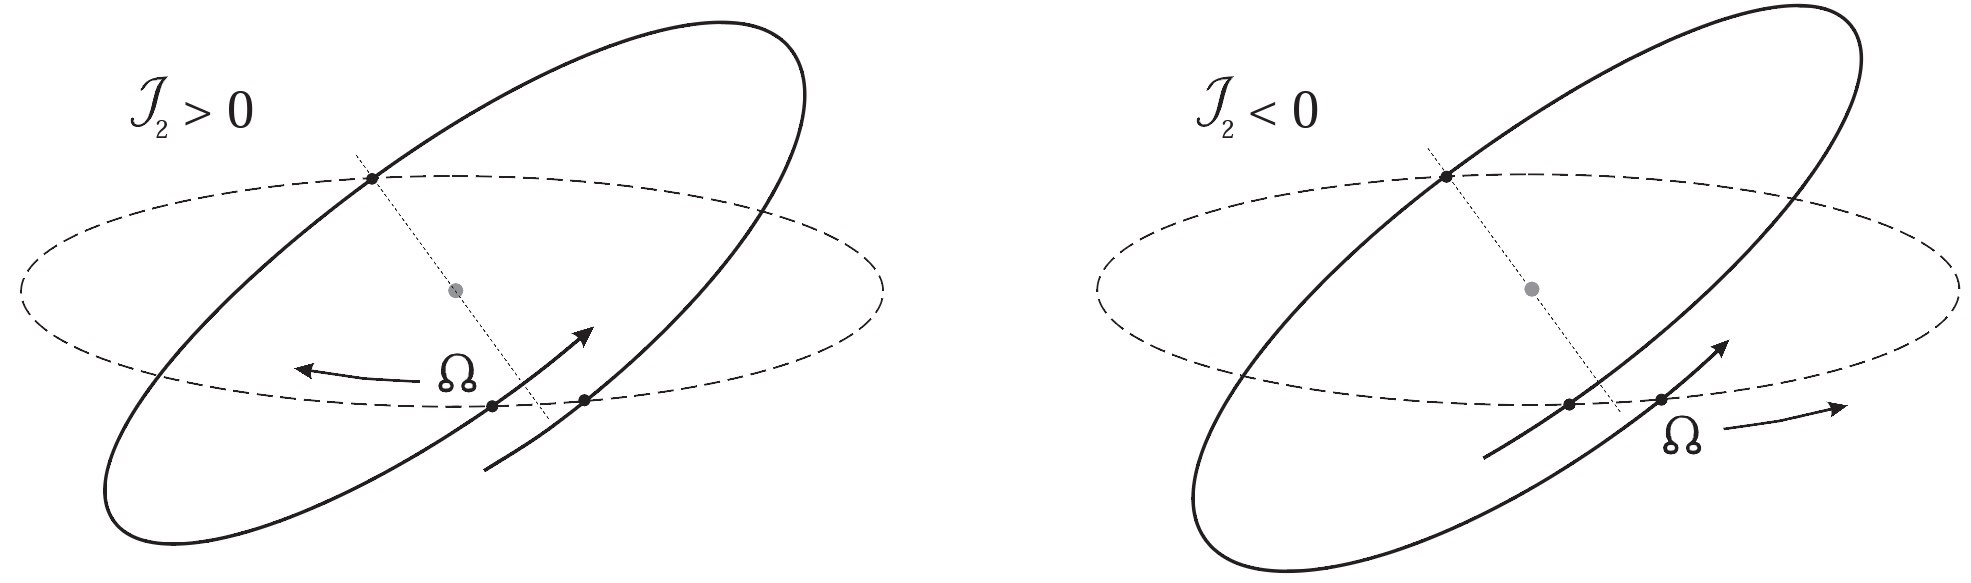
\includegraphics[height=0.4\textheight]{nodepert}\end{figure}

\end{frame}


\begin{wordonframe}{Perturbazioni periodiche/secolari}

$J_{\psi}$: costante del moto; $J_{\phi}$ e $J_{\chi}$: oscillazioni periodiche; $\phi$, $\chi$, $\psi$: oscillazioni periodiche sovrapposte a moto secolare. 

\end{wordonframe}



\part{Orbite non Kepleriane: problema dei 3 corpi.}\label{part:threebody}

\begin{frame}{this part toc}

\begin{itemize}

\item Problema dei 3 corpi

\end{itemize}


\end{frame}


\section{Problema dei 3 corpi: perturbazioni e problema ristretto}

\begin{frame}{Problema dei 3 corpi. Problema ristretto.}

\begin{itemize}
\item Terra-Sole-Giove
\item Terra-Sole-Luna
\item Giove-Saturno-Sole
\end{itemize}

\begin{block}{Problema ristretto}

\begin{columns}

\begin{column}{0.5\textwidth}

\begin{itemize}
\item Un corpa ha massa trascurabile risp. altri 2
\item Moto piano
\item Distanza tra i 2 primari costante
\end{itemize}

\end{column}


\begin{column}{0.5\textwidth}

Sole-Giove-Asteroide

Terra-Luna-Satellite artificiale

\begin{figure}

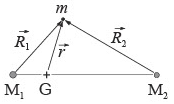
\includegraphics[keepaspectratio,width=0.6\textwidth]{3Brestrict}

\end{figure}

\end{column}

\end{columns}

\end{block}

\end{frame}

\begin{wordonframe}{Problema dei 3 corpi e problema ristretto}

\begin{align*}
&n_0a_0^3=G(M_1+M_2)
\end{align*}

Masse: $M_M\approx0.012$, $M_E=1$, $M_S\approx98$, $M_J\approx318$, $\msun{}\approx\num{3.3e5}$



Nel sistema Terra-Luna-Sole l'attrazione del Sole sulla Luna \'e una perturbazione nel sistema non inerziale che orbita attorno al Sole. 


\end{wordonframe}


\begin{frame}{Riferimento rotante}

\begin{columns}

\begin{column}{0.5\textwidth}

\begin{block}{Forza di Coriolis}
\begin{equation*}
\vec{f}_{cor}=-2m\vec{n}_0\wedge\dvec{r}
\end{equation*}
Lavoro nullo: ortogonale alla velocit\'a.

\end{block}

\end{column}

\begin{column}{0.5\textwidth}

\begin{block}{Forza centrifuga}
\begin{equation*}
\vec{f}_{cen}=-\nabla(-\frac{1}{2}m|\vec{n}_0\wedge\vec{r}|^2)
\end{equation*}
\'E conservativa.

\end{block}

\end{column}

\end{columns}

\begin{block}{Integrale di Jacobi}

\begin{equation*}
E=\frac{1}{2}m|\dvec{r}|^2-\frac{GM_1m}{R_1}-\frac{GM_2m}{R_2}-\frac{1}{2}m|\vec{n}_0\wedge\vec{r}|^2
\end{equation*}

\end{block}


\end{frame}

\begin{wordonframe}{Sistemi non inerziali, energia, forze conservative}

\begin{align*}
m\ddvec{x}=\vec{F}-m\dvec{\Omega}\wedge\vec{x}-2m\vec{\Omega}\wedge\dvec{x}-m\vec{\Omega}\wedge(\vec{\Omega}\wedge\vec{x})
\end{align*}

\end{wordonframe}

\begin{frame}{Regioni energeticamente permesse e punti di equilibrio}

\begin{columns}

\begin{column}{0.43\textwidth}

\begin{block}{Punti di equilibrio}

\begin{align*}
&\frac{1}{m}\nabla V=0\\
&=-n_0^2\vec{r}+\frac{GM_1}{R_1^3}\vec{R}_1+\frac{GM_2}{R_2^3}\vec{R}_2\\
&\vec{R}_1\nparallel\vec{R}_2:\\
&\vec{R}_1=\vec{R}_2=a_0 \Rightarrow L_4, L_5
\end{align*}

\end{block}


\end{column}

\begin{column}{0.57\textwidth}

\begin{block}{Superfici a velocit\'a nulla (di Hill)}

\begin{figure}[!t]

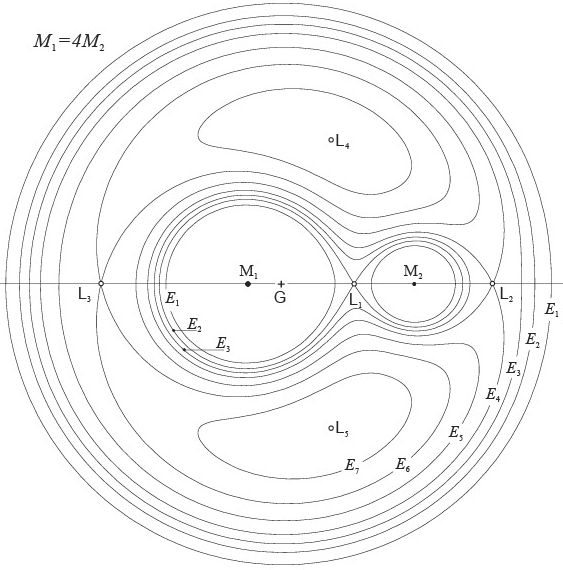
\includegraphics[keepaspectratio,width=0.9\textwidth]{hillzero}

\end{figure}

\end{block}

\end{column}

\end{columns}

Troiani

\end{frame}

\begin{wordonframe}{Superficie di Hill e punti Lagrangiani}

$L_1$, $L_2$, $L_3$: equilibrio instabile.

$L_4$, $L_5$: equilibrio stabile per $\frac{M_1}{M_2}>25$.

Oscillazioni attorno ai punti di equilibrio

\end{wordonframe}

\begin{frame}{Criterio Tisserand}

\begin{itemize}
\item $M_1\gg M_2$
\item $R_2$ a grandi distanze (cometa distante da Giove)
\end{itemize}

\begin{block}{Relazione di Tisserand}

\begin{equation*}
\frac{1}{2a}+\sqrt{\frac{a(1-e^2)}{a_0^3}}\cos{i}=const
\end{equation*}

\end{block}

\begin{block}{Velocit\'a relativa}

\begin{align*}
&v_{rel}=\frac{G\msun{}(3-T)}{a_0}\quad T=\frac{a_0}{2a}+\sqrt{\frac{a(1-e^2)}{a_0}}\cos{i}
\end{align*}

\end{block}

\end{frame}

\begin{wordonframe}{Criterio Tisserand}

a: semiasse cometa, $a_0$: semi-asse J, e,i eccentricit\'a inclinazione cometa

L'espressione connette gli elementi orbitali di una cometa (lontano da Giove) a pasaggi successivi.

Velocit\'a nel riferimento inerziale: $\TDy{t}{\vec{r}}=\dvec{r}+\vec{n}_0\wedge\vec{r}$.

\begin{align*}
&\vec{R}_1=\vec{r}+\frac{M_1}{M_1+M_2}\vec{a}_0\Rightarrow\TDy{t}{\vec{r}}=\TDy{t}{\vec{R}_1}-\frac{M_1}{M_1+M_2}\vec{n}_0\wedge\vec{a}_0\\
&E=E_1+c\\
&E_1=\frac{1}{2}|\TDy{t}{\vec{R}_1}|^2-\frac{GM_1}{R_1}-\frac{GM_2}{R_2}-\vec{n}_0\cdot\vec{R}_1\wedge\TDy{t}{\vec{R}_1}+\frac{M_1}{M_1+M_2}n_0^2\vec{a}_0\cdot\vec{R}_1
\end{align*}

Gli ultimi 2 termini descrivono variazione energetiche dovute ad azione cometa su Sole e Jupiter; in approx $M_1\gg M_2$: $E_1\approx E_c-\vec{n}_0\cdot\vec{J}_c$

\end{wordonframe}

\begin{wordonframe}{Velocit\'a relativa J-comet}
($r\approx a_G$)
\begin{align*}
&v_{\theta}=\frac{h}{a_G}=\sqrt{\frac{G\msun{}}{a_G}}\sqrt{\frac{a_c(1-e_c^2)}{a_G}}\\
&v^2=G\msun{}[\frac{2}{a_G}-\frac{1}{a_c}]\\
&v_{rev}=v^2-v_{\theta}^2=\frac{G\msun{}}{a_G}[3-\frac{a_G}{a_c}-2\cos{i}\sqrt{(1-e_c^2)\frac{a_c}{a_G}}]
\end{align*}

\end{wordonframe}

\begin{frame}{Problema 3 corpi ristretto: integrali primi}

\begin{columns}[T]

\begin{column}{0.5\textwidth}

\begin{block}{sistema a 2 gradi di libert\'a}

Sistema a 2 gradi di libert\'a ha 3 integrali primi.

\end{block}

\end{column}

\begin{column}{0.5\textwidth}

\begin{block}{Integrali primi uniformi}
Integrali primi continui
\end{block}

\begin{block}{Analiticit\'a}

$\epsilon=\frac{M_2}{M_1}$ ($\epsilon=0$: problema a 2 corpi)

\end{block}

\end{column}

\end{columns}

\begin{block}{Poincar\'e (1890)}

Il problema dei 3 corpi ristretto ha solo l'integrale di Jacobi come integrale uniforme e analitico in $\epsilon$.

\end{block}

Il problema a 3 corpi (ristretto non \'e integrabile)

\begin{block}{Comportamento caotico}

\begin{columns}[T]

\begin{column}{0.5\textwidth}
Conoscenza condizioni iniziali con precisione finita
\end{column}

\begin{column}{0.5\textwidth}
Divergenza esponenziale delle traiettorie nello spazio delle fasi.
\end{column}

\end{columns}

\end{block}

\end{frame}

\begin{wordonframe}{Integrali primi}

\begin{columns}[T]
\begin{column}{0.5\textwidth}
\begin{align*}
&x(0),y(0)\\
&\dot{x}(0),\dot{y}(0)
\end{align*}
\end{column}

\begin{column}{0.5\textwidth}
Soluzione equazione del moto: Curva nello spazio delle fasi $F(x,y)=c$.
\end{column}

\end{columns}

Sistema integrabile a n-dof: n variabili angolo $\phi_i$ (variano linearmente nel tempo), n variabili azione (costanti del moto)

\begin{block}{Liuville-Arnol'd}
Una traiettoria di fase \'e densa nel suo toro n-dimensionale
\end{block}

\end{wordonframe}


\begin{frame}{Problema a 3 corpi: disuguaglianza di Easton}

Sistema legato di n punti materiale con baricentro fermo.

\begin{columns}[T]

\begin{column}{0.5\textwidth}
\begin{equation*}
IV^2\geq2|E|J^2
\end{equation*}
\end{column}

\begin{column}{0.5\textwidth}
$2|E|J^2$: costante del moto (Integrale di Zare).

$IV^2$: dipende dalla configurazione del sistema e non dalla velocit\'a

\end{column}

\end{columns}


\end{frame}



\end{document}